% Provenance (never printed): see sources/outline_sources.md (Year 1: decay systems K-Ar,
% Rb-Sr, U-Pb and radiocarbon; closure temperature; dating sedimentary sequences with
% volcanic ashes; calibrating the scale). Exercise and problem values in the Book 3
% scratch calculator calc/ch25.py; figures from figdata/bachelor-1/decay_curves.py,
% isochron.py and radiocarbon.py (IntCal20, dataset bachelor-1-intcal20).
% The decay law, half-life and decay constant belong to the physics series (recalled);
% the closed system and the isochron of minerals are Book 2's (g12 age-of-the-earth),
% re-founded here with whole-rock samples and least squares. The concordia diagram and
% thermochronology are the Year 3 volume's: prose pointers only. Mass spectrometry is
% the chemistry series' (recalled). The isochron figure uses an invented rhyolite so that
% the Varden granite of the problem is not solved in the course.
\chapter{रेडियोमेट्रिक आयु-निर्धारण की विधियाँ}\label{ch:b1:radiometric-methods}

2001 में पश्चिमी ऑस्ट्रेलिया की जैक हिल्स के डेट्राइटल ज़िरकॉन कणों पर काम करती एक टीम ने एक ऐसे कण की रिपोर्ट दी जो \num[uncertainty-mode=separate]{4404 \pm 8} दस लाख वर्ष पहले क्रिस्टलित हुआ था। बाद के काम ने इन कणों की आयु की पुष्टि की: वे पृथ्वी पर बने किसी भी प्रकार के ज्ञात सबसे पुराने पदार्थ हैं, और दिखाते हैं कि सौरमंडल के जन्म के लगभग 160 मिलियन वर्षों के भीतर एक परत बन चुकी थी। दूसरे छोर पर, आर्गन आयुओं ने क्रिटेशियस के अंत के विलोपन को \qty{66.00}{\Ma} पूर्व रखा है, उस प्रभाव के \num{32000} वर्षों के भीतर जिसे उसका कारण माना जाता है। दोनों संख्याएँ परमाणुओं की गिनती से आती हैं: एक रेडियोधर्मी जनक जो ज्ञात दर से क्षय होता है, और एक संतति जो जमा होती है। यह अध्याय बताता है कि ऐसी घड़ियाँ कैसे पढ़ी जाती हैं, हर एक अलग घटना को क्यों आँकती है, और वे \cref{ch:b1:stratigraphic-scale} के चार्ट को वर्षों के पैमाने पर कैसे टाँगती हैं।
% ledger: wilde01:4404, uw14:jack-hills, ics:base.Paleogene, renne:kpg

\begin{omfigure}
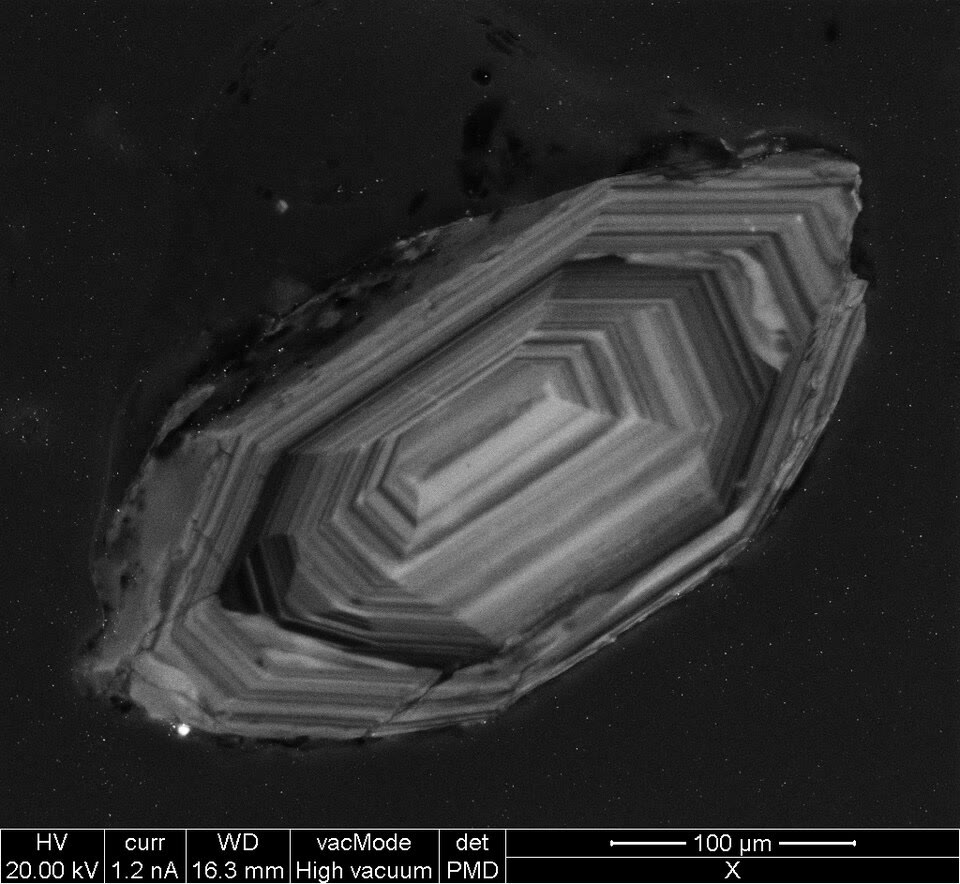
\includegraphics[width=0.5\linewidth]{images/book3/b1-zircon-cl.jpg}

{\small एक ज़िरकॉन कण, लगभग एक मिलीमीटर के एक-तिहाई लंबा, स्कैनिंग इलेक्ट्रॉन सूक्ष्मदर्शी के इलेक्ट्रॉन-पुंज के नीचे उसके उत्सर्जित प्रकाश (कैथोडोल्यूमिनेसेंस) से चित्रित। क्रिस्टल के फलकों का अनुसरण करने वाली पट्टियाँ थोड़ी भिन्न संघटन के क्षेत्र हैं, जो उसके बढ़ते समय एक के बाद एक जमे। यह कण एक बलुआ पत्थर से चुना गया था, इसलिए वह बलुआ पत्थर से पुराना है: वह उस चट्टान की आयु बताता है जिससे वह अपरदित हुआ। (फ़ोटो: Emmanuel Roquette, CC~BY-SA~4.0, विकिमीडिया कॉमन्स के माध्यम से।)}
\label{fig:b1:radiometric-methods:zircon}
\end{omfigure}
% ledger: commons:zircon-cl

\begin{recall}
भौतिकी खंड रेडियोधर्मी क्षय का वर्णन करते हैं: किसी रेडियोधर्मी समस्थानिक के नाभिक यादृच्छिक रूप से, तापमान और दाब से स्वतंत्र, क्षय होते हैं, इसलिए बचा हुआ $N$, समय $t$ के बाद, $N = N_0\,e^{-\lambda t}$ के अनुसार घटता है, जहाँ $\lambda$ क्षय-स्थिरांक है; अर्ध-आयु $T = \ln 2/\lambda$ है। किसी तत्व के समस्थानिकों में प्रोटॉनों की संख्या समान और न्यूट्रॉनों की संख्या भिन्न होती है; रसायन-विज्ञान के खंड द्रव्यमान-स्पेक्ट्रोमीटर का वर्णन करते हैं, जो आयनों को द्रव्यमान से छाँटता है। पुस्तक~2, कक्षा~12 में, वह चट्टान या \omterm{def:b1:rock-forming-minerals:mineral}{खनिज} जिसने अपने परिवेश के साथ कोई जनक या संतति परमाणु नहीं बदले, एक बंद तंत्र है, और वार्डेन ग्रेनाइट के \omterm{def:b1:rock-forming-minerals:mineral}{खनिज}, रूबिडियम–स्ट्रॉन्शियम \omterm{def:b1:radiometric-methods:isochron}{समतापरेखा} पर रखे गए, 310 मिलियन वर्ष की आयु दी। बायोटाइट, मस्कोवाइट और हॉर्नब्लेंड \cref{def:b1:rock-forming-minerals:groups} के \omterm{def:b1:rock-forming-minerals:groups}{अभ्रक} और \omterm{def:b1:rock-forming-minerals:groups}{एम्फ़ीबोल} हैं। दो आँके गए स्तरों के बीच की आयु प्रक्षेपित की जा सकती है (\cref{prop:b1:stratigraphic-scale:interpolation})।
\end{recall}
% ledger: tulane:radiometric, villa22:rb87

\section{क्षय-तंत्र}\label{sec:b1:radiometric-methods:systems}

आयु-निर्धारण के लिए एक घड़ी को दो गिनतियाँ चाहिए: जनक में क्या बचा है, और घड़ी चलने से लेकर अब तक उसने कितनी संतति बनाई है।

\begin{definition}[जनक समस्थानिक, रेडियोजनित संतति]\label{def:b1:radiometric-methods:radiogenic}
आयु-निर्धारण में प्रयुक्त एक क्षय-तंत्र में \emph{जनक समस्थानिक}\index{जनक समस्थानिक} वह रेडियोधर्मी समस्थानिक है जिसका क्षय घड़ी का काम करता है, और संतति वह समस्थानिक है जो उसके क्षय से बनता है। \emph{रेडियोजनित संतति}\index{रेडियोजनित संतति}, $D^*$ लिखी जाती है, संतति का वह भाग है जो नमूने के भीतर जनक के क्षय से तब बना जब से घड़ी चली; शेष, $D_0$, आरंभ से वहाँ था। आज मापी गई संतति के परमाणुओं की संख्या $D = D_0 + D^*$ है।
\end{definition}

\begin{proposition}[रेडियोजनित वृद्धि और आयु-समीकरण]\label{prop:b1:radiometric-methods:growth}
एक बंद तंत्र में, जिसमें आज जनक के $P$ परमाणु हैं, समय $t$ में बनी \omterm{def:b1:radiometric-methods:radiogenic}{रेडियोजनित संतति}
\[
  D^* = P\,\bigl(e^{\lambda t} - 1\bigr),
\]
यदि हर क्षय संतति का एक परमाणु देता है। तब आयु है
\[
  t = \frac{1}{\lambda}\,\ln\!\left(1 + \frac{D^*}{P}\right).
\]
\end{proposition}

\begin{proof}
क्षय-नियम से जनक घड़ी के आरंभ पर $P_0 = P\,e^{\lambda t}$ था। एक बंद तंत्र में हर लुप्त जनक परमाणु एक संतति परमाणु बन गया है, इसलिए $D^* = P_0 - P = P\,(e^{\lambda t} - 1)$। तब $e^{\lambda t} = 1 +
D^*/P$; लघुगणक लेने पर आयु मिलती है।
\end{proof}

आयु केवल दो परमाणु-संख्याओं के अनुपात पर निर्भर करती है, जिसे द्रव्यमान-स्पेक्ट्रोमीटर सबसे अच्छा मापता है। नीचे का चित्र दोनों गिनतियाँ अर्ध-आयु की इकाइयों में दिखाता है: एक अर्ध-आयु के बाद $D^*/P = 1$, दो के बाद $3$, तीन के बाद $7$ --- सामान्यतः $2^n - 1$, $n$ अर्ध-आयुओं के बाद।

\begin{omfigure}
\begin{tikzpicture}
\begin{axis}[omrecord, width=0.72\linewidth, height=5.6cm, xmin=0, xmax=5, ymin=0, ymax=1.05,
  xlabel={समय (अर्ध-आयु)}, ylabel={आरंभिक जनक का अंश},
  xtick={0,1,...,5}, ytick={0,0.25,0.5,0.75,1}]
% computed in figdata/bachelor-1/decay_curves.py (no real-world number)
\addplot[omThm, line width=1pt] table[x=n, y=P] {figdata/out/bachelor-1-decay_curves-curves.dat};
\addplot[omDef, line width=1pt] table[x=n, y=D] {figdata/out/bachelor-1-decay_curves-curves.dat};
\addplot[only marks, mark=*, mark size=1.4pt, black!60] table[x=n, y=P] {figdata/out/bachelor-1-decay_curves-marks.dat};
\addplot[only marks, mark=*, mark size=1.4pt, black!60] table[x=n, y=D] {figdata/out/bachelor-1-decay_curves-marks.dat};
\node[font=\small, text=omThm, anchor=south west] at (axis cs:0.35,0.80) {जनक $P$};
\node[font=\small, text=omDef, anchor=north west] at (axis cs:2.55,0.66) {रेडियोजनित संतति $D^*$};
\node[font=\scriptsize, anchor=west, inner sep=1pt] (r1) at (axis cs:0.12,0.5) {$D^*/P = 1$};
\draw[black!60, line width=0.4pt] (r1.east) -- (axis cs:0.95,0.5);
\node[font=\scriptsize, anchor=south] at (axis cs:2,0.77) {$3$};
\node[font=\scriptsize, anchor=south] at (axis cs:3,0.89) {$7$};
\node[font=\scriptsize, anchor=north] at (axis cs:4,0.915) {$15$};
\node[font=\scriptsize, anchor=north east] at (axis cs:4.97,0.95) {$31$};
\end{axis}
\end{tikzpicture}

{\small एक बंद तंत्र में जनक और उसकी \omterm{def:b1:radiometric-methods:radiogenic}{रेडियोजनित संतति}, जनक परमाणुओं की आरंभिक संख्या के अंशों के रूप में, अर्ध-आयु की इकाइयों में गिने गए समय के विरुद्ध। उनका योग एक के बराबर रहता है; अनुपात $D^*/P$, जो हर पूर्ण अर्ध-आयु पर छपा है, हर चरण पर दोगुना होकर एक जोड़ता है।}
\label{fig:b1:radiometric-methods:decay}
\end{omfigure}

एक घड़ी आयुओं की एक खिड़की के भीतर ही ठीक पढ़ी जाती है। एक अर्ध-आयु से बहुत पहले संतति जनक का एक छोटा अंश है; कई अर्ध-आयुओं के बाद मापने के लिए बहुत कम जनक बचता है। नीचे की सारणी सबसे अधिक प्रयुक्त तंत्रों को, उन पदार्थों के साथ जिन पर हर एक लगाया जाता है, सूचीबद्ध करती है।

\begin{table}[ht]
\centering
\small
\renewcommand{\arraystretch}{1.25}
\begin{tabular}{|l|l|c|c|>{\raggedright\arraybackslash}p{4.3cm}|}
\hline
जनक & संतति & अर्ध-आयु (वर्ष) & $\lambda$ (प्रति वर्ष) & आयु-निर्धारित पदार्थ \\
\hline
$^{14}\mathrm{C}$ & $^{14}\mathrm{N}$ & \num{5700} & \num{1.216e-4} & लकड़ी, कोयला, हड्डी, सीप \\
$^{40}\mathrm{K}$ & $^{40}\mathrm{Ar}$, $^{40}\mathrm{Ca}$ & \num{1.25e9} & \num{5.543e-10} & पोटैशियम-समृद्ध \omterm{def:b1:rock-forming-minerals:mineral}{खनिज}: सैनिडीन, बायोटाइट, हॉर्नब्लेंड \\
$^{87}\mathrm{Rb}$ & $^{87}\mathrm{Sr}$ & \num{4.96e10} & \num{1.3972e-11} & ग्रेनाइट (संपूर्ण शैलें), \omterm{def:b1:rock-forming-minerals:groups}{अभ्रक} \\
$^{147}\mathrm{Sm}$ & $^{143}\mathrm{Nd}$ & \num{1.07e11} & \num{6.46e-12} & शैलें और उनके \omterm{def:b1:rock-forming-minerals:mineral}{खनिज} (समतापरेखाएँ) \\
$^{235}\mathrm{U}$ & $^{207}\mathrm{Pb}$ & \num{7.04e8} & \num{9.8485e-10} & ज़िरकॉन \\
$^{238}\mathrm{U}$ & $^{206}\mathrm{Pb}$ & \num{4.47e9} & \num{1.55125e-10} & ज़िरकॉन \\
\hline
\end{tabular}
\caption{मुख्य क्षय-तंत्र। पोटैशियम-40 और दो यूरेनियमों के क्षय-स्थिरांक आयु परिकलन के लिए प्रयुक्त पारंपरिक मान हैं; रूबिडियम-87 और समैरियम-147 के स्थिरांक अर्ध-आयुओं से परिकलित हैं, और कार्बन-14 का स्थिरांक उसकी \num{5700} वर्ष की अर्ध-आयु से।}
\label{tab:b1:radiometric-methods:systems}
\end{table}
% ledger: iaea:c14, iaea:k40-branches, amherst:constants, villa22:rb87, iaea:sm147, iaea:isotopes, tulane:kar, tulane:upb-zircon, tulane:c14

दो प्रकार के संख्यात्मक मान एक ही नाभिकों के लिए प्रयोग में हैं, और एक आयु को बताना चाहिए कि उसने कौन सा उपयोग किया। परमाणु-आँकड़ों की तालिकाएँ पोटैशियम-40 की अर्ध-आयु \num{1.248e9} वर्ष देती हैं और उसके क्षयों का \qty{10.72}{\percent} आर्गन की ओर भेजती हैं; भू-कालिकी में पारंपरिक रूप से प्रयुक्त स्थिरांक $\lambda = \num{5.543e-10}$ प्रति वर्ष देते हैं (अर्ध-आयु \num{1.2505e9} वर्ष), और $0.581/5.543 = \qty{10.48}{\percent}$ क्षयों को आर्गन की ओर भेजते हैं। रेडियोकार्बन आयुएँ, जैसा \cref{sec:b1:radiometric-methods:kar} समझाता है, \num{5568} वर्ष की अर्ध-आयु से परिकलित होती हैं, जिसे बहुत छोटा जाना जाता है। अंतर कुछ प्रतिशत तक पहुँचते हैं, जो सर्वोत्तम आयुओं के \qty{0.01}{\percent} से कहीं अधिक हैं (\cref{sec:b1:radiometric-methods:sediments})। पोटैशियम-40 का अनिश्चित क्षय-स्थिरांक स्वयं, दो शाखाओं और लंबी अर्ध-आयु वाला नाभिक, उसकी आयुओं की सटीकता सीमित करता है।
% ledger: iaea:k40-branches, amherst:constants, sp77:conventional-age, ics:base.Triassic, nmgrl:arar

\begin{proposition}[आयु की सटीकता]\label{prop:b1:radiometric-methods:precision}
यदि अनुपात $R = D^*/P$ मानक अनिश्चितता $\sigma_R$ के साथ मापा जाए, तो आयु यह अनिश्चितता रखती है
\[
  \sigma_t = \frac{\sigma_R}{\lambda\,(1 + R)}.
\]
\end{proposition}

\begin{proof}
एक छोटी त्रुटि $\delta R$ के लिए, आयु $t = \ln(1+R)/\lambda$ इतनी बदलती है: $\delta t = t'(R)\,\delta R = \delta R/\bigl(\lambda(1 + R)\bigr)$।
\end{proof}

युवा नमूने के लिए $R$ छोटा है और $\sigma_t \approx \sigma_R/\lambda$: आयु की निरपेक्ष त्रुटि इससे तय होती है कि थोड़ी संतति कितनी अच्छी मापी जा सकती है। लंबी अर्ध-आयु (छोटा $\lambda$) उसे बढ़ाती है। इसी लिए रूबिडियम–स्ट्रॉन्शियम और यूरेनियम–सीसा लगभग दस मिलियन वर्ष से पुरानी चट्टानों के लिए काम आते हैं, जबकि पोटैशियम–आर्गन लगभग दस हज़ार वर्ष तक की युवा चट्टानों तक पहुँचता है, और रेडियोकार्बन पिछले \num{70000} वर्ष को ढकता है।
% ledger: tulane:ranges

\section{समतापरेखाएँ}\label{sec:b1:radiometric-methods:isochrons}

आयु-समीकरण को $D^*$ चाहिए, पर यंत्र $D = D_0 + D^*$ मापता है, और $D_0$ शायद ही कभी शून्य है: स्ट्रॉन्शियम-87 हर उस \omterm{def:b1:rock-forming-minerals:mineral}{खनिज} में मौजूद है जिसने अपने बनते समय स्ट्रॉन्शियम लिया। \omterm{def:b1:radiometric-methods:isochron}{समतापरेखा} कई नमूनों को मापकर $D_0$ हटाती है, जो संतति तत्व के एक ही समस्थानिक-संघटन से आरंभ हुए थे।

\begin{definition}[समतापरेखा, आरंभिक अनुपात]\label{def:b1:radiometric-methods:isochron}
मान लीजिए $S$ संतति तत्व का एक स्थायी समस्थानिक है जिसे कोई क्षय उत्पन्न नहीं करता ($^{86}\mathrm{Sr}$ स्ट्रॉन्शियम के लिए, $^{144}\mathrm{Nd}$ नियोडिमियम के लिए)। एक \emph{समतापरेखा}\index{समतापरेखा} वह सीधी रेखा है जिस पर, $y = D/S$ बनाम $x = P/S$ के आलेख में, वे नमूने आलेखित होते हैं जो एक ही समय पर, एक ही $D/S$ मान के साथ बने और तब से बंद तंत्र रहे हैं। वह साझा आरंभिक मान $y_0 = (D/S)_0$ \emph{आरंभिक अनुपात}\index{आरंभिक अनुपात} है।
\end{definition}
% ledger: tulane:radiometric, tulane:c14

\begin{theorem}[समतापरेखा]\label{thm:b1:radiometric-methods:isochron}
वे नमूने जो एक ही समय पर, एक ही \omterm{def:b1:radiometric-methods:isochron}{आरंभिक अनुपात} $y_0$ के साथ बने, और समय $t$ के लिए बंद तंत्र रहे हैं, संतुष्ट करते हैं
\[
  y = y_0 + \bigl(e^{\lambda t} - 1\bigr)\,x .
\]
उनके बिंदु ढलान $m = e^{\lambda t} - 1$ और अंतःखंड $y_0$ की एक सीधी रेखा पर होते हैं, और $t = \ln(1+m)/\lambda$।
\end{theorem}

\begin{proof}
हर नमूने के लिए, \cref{prop:b1:radiometric-methods:growth} से $D = D_0 + P\,(e^{\lambda t} - 1)$। $S$ के परमाणुओं की संख्या नहीं बदली है, क्योंकि $S$ स्थायी है, किसी क्षय से नहीं बनता, और तंत्र बंद है; उससे भाग देने पर $y = y_0 + (e^{\lambda t} - 1)\,x$ मिलता है, जिसमें $y_0$ परिकल्पना से सभी नमूनों के लिए एक ही है।
\end{proof}

जब एक ग्रेनाइट क्रिस्टलित हुआ, तो उसके सभी नमूनों का $y_0$ एक ही था और वे एक क्षैतिज रेखा पर आलेखित होते; तब से हर एक अपने $x$ के अनुपात में ऊपर खिसका है, और रेखा अपने अंतःखंड के चारों ओर घूमी है। ढलान को अच्छी तरह परिभाषित करने के लिए नमूनों को भिन्न $x$ मान चाहिए: अधिक और कम रूबिडियम वाले \omterm{def:b1:rock-forming-minerals:mineral}{खनिज}, जैसा पुस्तक~2 में था, या एक ही अंतर्वेधन के अधिक और कम विकसित भागों से लिए गए संपूर्ण-शैल नमूने। रेखा से हटा बिंदु वह नमूना है जो बंद नहीं था, या जिसने \omterm{def:b1:radiometric-methods:isochron}{आरंभिक अनुपात} साझा नहीं किया। \omterm{def:b1:radiometric-methods:isochron}{आरंभिक अनुपात} स्वयं एक अनुरेखक है: मैंटल से आया मैग्मा एक निम्न $^{87}\mathrm{Sr}/^{86}\mathrm{Sr}$ लेता है, लगभग $0.7025$, और पिघली महाद्वीपीय पपड़ी से बना एक उच्च, लगभग $0.710$, क्योंकि पपड़ी रूबिडियम से समृद्ध है और युगों में उसने अधिक स्ट्रॉन्शियम-87 बनाया है।
% ledger: tulane:radiometric, tulane:sr-initial

वास्तविक बिंदु कभी ठीक रेखा पर नहीं पड़ते। रेखा का सामान्य अनुमान वह है जो बिंदुओं की उससे ऊर्ध्वाधर दूरियों के वर्गों को यथासंभव छोटा बनाता है।

\begin{proposition}[न्यूनतम-वर्ग रेखा]\label{prop:b1:radiometric-methods:lsq}
मान लीजिए $(x_i, y_i)$, $i = 1, \dots, n$, कम से कम दो भिन्न $x_i$ वाले बिंदु हैं, जिनके माध्य $\bar x$ और $\bar y$ हैं, और मान लीजिए
\[
  S_{xx} = \sum_i (x_i - \bar x)^2, \qquad S_{xy} = \sum_i (x_i - \bar x)(y_i - \bar y).
\]
वह रेखा $y = b + m x$ जो $Q(b, m) = \sum_i (y_i - b - m x_i)^2$ को न्यूनतम करती है, उसकी है
\[
  m = \frac{S_{xy}}{S_{xx}}, \qquad b = \bar y - m\,\bar x ,
\]
और केंद्रक $(\bar x, \bar y)$ से गुज़रती है।
\end{proposition}

\begin{proof}
$Q$ बिंदुओं पर वर्गों का योग है, $(b, m)$ में दूसरी घात का एक बहुपद जो हर दिशा में अनंत की ओर जाता है, इसलिए वह न्यूनतम तक वहाँ पहुँचता है जहाँ दोनों आंशिक अवकलज शून्य हों। $\partial Q/\partial b = -2 \sum_i (y_i - b - m x_i) = 0$ से $n\bar y = n b + n m \bar x$ मिलता है, इसलिए $b = \bar y - m \bar x$: रेखा केंद्रक से गुज़रती है। प्रतिस्थापित करने पर, $y_i - b - m x_i = (y_i - \bar y) - m(x_i -
\bar x)$, और $\partial Q/\partial m = -2 \sum_i x_i \bigl[(y_i - \bar y) - m(x_i
- \bar x)\bigr] = 0$। चूँकि $\sum_i (y_i - \bar y) = \sum_i (x_i - \bar x) = 0$ है, इस योग में $x_i$ को $x_i - \bar x$ से बदला जा सकता है, जो $S_{xy} - m S_{xx} = 0$ देता है। $S_{xx} > 0$ है क्योंकि सभी $x_i$ समान नहीं हैं।
\end{proof}

बिंदुओं का रेखा के चारों ओर बिखराव ढलान की अनिश्चितता देता है। अवशेषों $r_i = y_i - b - m x_i$ के साथ, बिखराव का मानक विचलन $s = \sqrt{\sum_i r_i^2/(n-2)}$ है --- दो प्राचल दो स्वतंत्रता-कोटियाँ लेते हैं --- और ढलान तथा अंतःखंड की मानक अनिश्चितताएँ
\[
  \sigma_m = \frac{s}{\sqrt{S_{xx}}}, \qquad
  \sigma_b = s\,\sqrt{\frac1n + \frac{\bar x^2}{S_{xx}}} .
\]
ये सांख्यिकी के दो परिणाम यहाँ स्वीकार किए जाते हैं; तब आयु $\sigma_t = \sigma_m/\bigl(\lambda(1 + m)\bigr)$ वहन करती है, \cref{prop:b1:radiometric-methods:precision} के तर्क से। वे दिखाते हैं कि एक अच्छी \omterm{def:b1:radiometric-methods:isochron}{समतापरेखा} क्या बनाती है: बहुत से बिंदु, $x$ में व्यापक रूप से फैले (एक बड़ा $S_{xx}$), और थोड़े बिखराव के साथ।

\begin{method}[समतापरेखा का अनुरूपण]\label{met:b1:radiometric-methods:isochron}
\begin{enumerate}
  \item एक ही पिंड के कम से कम चार नमूनों में $x = P/S$ और $y = D/S$ मापिए, जो $x$ को यथासंभव व्यापक रूप से फैलाने के लिए चुने गए हों।
  \item उन्हें आलेखित कीजिए; प्रवृत्ति से स्पष्ट रूप से हटे किसी भी बिंदु को, कारण सहित, अलग रखिए।
  \item $\bar x$, $\bar y$, $S_{xx}$, $S_{xy}$ परिकलित कीजिए, फिर $m = S_{xy}/S_{xx}$ और $b = \bar y - m \bar x$।
  \item अवशेष, $s$, $\sigma_m$ और $\sigma_b$ परिकलित कीजिए।
  \item आयु $t = \ln(1+m)/\lambda$ है, $\sigma_t =
        \sigma_m/\bigl(\lambda(1+m)\bigr)$ के साथ; \omterm{def:b1:radiometric-methods:isochron}{आरंभिक अनुपात} $b \pm \sigma_b$ है।
\end{enumerate}
\end{method}

\begin{example}[एक आविष्कृत राइओलाइट]\label{ex:b1:radiometric-methods:rhyolite}
एक राइओलाइट लावा-श्रृंखला के छह संपूर्ण-शैल नमूने (अभ्यास का डेटा) देते हैं:
\begin{center}
\small
\begin{tabular}{|l|cccccc|}
\hline
$x = {}^{87}\mathrm{Rb}/^{86}\mathrm{Sr}$ & 1.85 & 4.62 & 9.30 & 14.75 & 21.20 & 27.60 \\
$y = {}^{87}\mathrm{Sr}/^{86}\mathrm{Sr}$ & 0.71732 & 0.73332 & 0.76164 & 0.79420 & 0.83226 & 0.87028 \\
\hline
\end{tabular}
\end{center}
यहाँ $\bar x = 13.22$, $\bar y = 0.784837$, $S_{xx} = 491.41$ और $S_{xy} = 2.92308$, इसलिए $m = 0.0059484$ और $b = 0.70620$। अवशेष देते हैं $s = 0.00024$, $\sigma_m = \num{1.10e-5}$ और $\sigma_b = 0.00018$। आयु है $t = \ln(1.0059484)/\num{1.3972e-11} = \qty{424.5}{\Ma}$, जिसकी $\sigma_t = \num{1.10e-5}/(\num{1.3972e-11} \times 1.0059) = \qty{0.8}{\Myr}$ है: \qty[uncertainty-mode=separate]{424.5(8)}{\Ma}, \omterm{def:b1:radiometric-methods:isochron}{आरंभिक अनुपात} \num[uncertainty-mode=separate]{0.70620(18)} (नीचे का चित्र)।
\end{example}
% values: isochron.py (slope 0.005948361, intercept 0.7061993, age 424.4732, sigma 0.7827871); ledger: villa22:rb87

\begin{omfigure}
\begin{tikzpicture}
\begin{axis}[omrecord, width=0.74\linewidth, height=6cm, xmin=0, xmax=30, ymin=0.70, ymax=0.88,
  xlabel={$^{87}\mathrm{Rb}/^{86}\mathrm{Sr}$}, ylabel={$^{87}\mathrm{Sr}/^{86}\mathrm{Sr}$},
  ytick={0.70,0.72,...,0.88},
  y tick label style={/pgf/number format/.cd, fixed, fixed zerofill, precision=2}]
% computed in figdata/bachelor-1/isochron.py (exercise data, invented rhyolite); ledger: villa22:rb87
\addplot[black!60, densely dotted, line width=0.7pt] table[x=x, y=y] {figdata/out/bachelor-1-isochron-initial.dat};
\addplot[omDef, line width=0.9pt] table[x=x, y=y] {figdata/out/bachelor-1-isochron-line.dat};
\addplot[omThm, only marks, mark=*, mark size=2pt] table[x=x, y=y] {figdata/out/bachelor-1-isochron-points.dat};
\node[font=\scriptsize, text=omDef, anchor=south east, align=right] at (axis cs:19,0.83)
  {न्यूनतम-वर्ग ढलान $0.005948$\\ आयु \qty[uncertainty-mode=separate]{424.5(8)}{\Ma}};
\node[font=\scriptsize, text=black!70, anchor=south west] at (axis cs:9,0.7068)
  {आरंभिक अनुपात $0.70620$, जब लावा बने};
\end{axis}
\end{tikzpicture}

{\small एक आविष्कृत राइओलाइट के छह संपूर्ण-शैल नमूनों की रूबिडियम–स्ट्रॉन्शियम \omterm{def:b1:radiometric-methods:isochron}{समतापरेखा} (अभ्यास का डेटा)। बिंदु न्यूनतम-वर्ग रेखा के चारों ओर थोड़े बिखरे हैं, जो उनके केंद्रक से गुज़रती है; धराशायी रेखा वह है जहाँ वे सभी लावा के बनने के समय थे।}
\label{fig:b1:radiometric-methods:isochron}
\end{omfigure}

\begin{inthelab}[समस्थानिकों का तौलना]
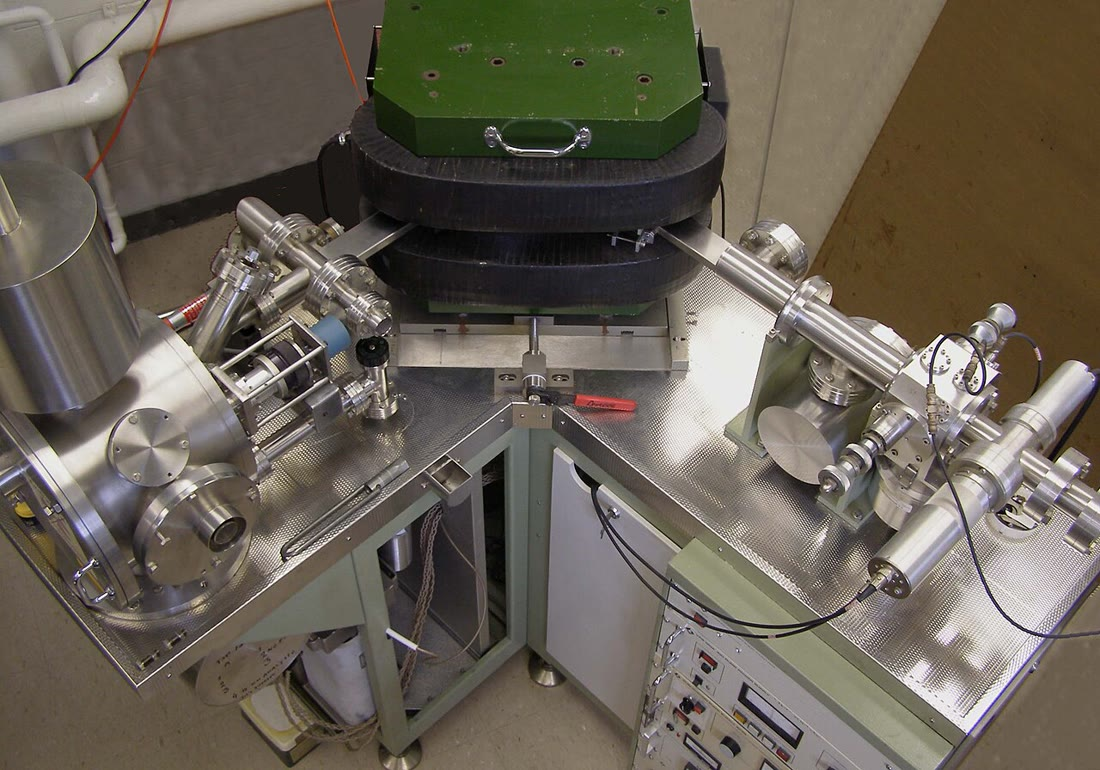
\includegraphics[width=0.42\linewidth]{images/book3/b1-tims.jpg}\hfill
\begin{minipage}[b]{0.55\linewidth}
एक तापीय-आयनन द्रव्यमान-स्पेक्ट्रोमीटर (बायीं ओर) स्ट्रॉन्शियम जैसे तत्वों के समस्थानिक-अनुपात मापता है। तत्व, जो रसायन विधि से घुले नमूने से अलग किया गया है, निर्वात में एक धातु के तंतु पर लादा जाता है; गरम होने पर वह आयन छोड़ता है, जो एक बड़े विद्युत-चुंबक के क्षेत्र (केंद्र की काली कुंडलियाँ) से त्वरित और मोड़े जाते हैं, हल्के आयन भारी आयनों से अधिक, ताकि हर समस्थानिक अपने संग्राहक तक पहुँचे। समस्थानिकों के अनुपात वही हैं जो यंत्र सबसे अच्छा मापता है, और इसी लिए केवल अनुपातों पर आधारित विधियाँ सबसे सटीक हैं। (फ़ोटो: Radiogenic, CC0, विकिमीडिया कॉमन्स के माध्यम से।)
\end{minipage}
\end{inthelab}
% ledger: commons:tims, amherst:constants

\section{पोटैशियम–आर्गन, यूरेनियम–सीसा और रेडियोकार्बन}\label{sec:b1:radiometric-methods:kar}

\subsection*{एक जनक, दो संतति}

\begin{definition}[शाखित क्षय]\label{def:b1:radiometric-methods:branching}
किसी जनक का \emph{शाखित क्षय}\index{शाखित क्षय} होता है जब उसके नाभिक दो या अधिक मार्गों से भिन्न संततियों में क्षय होते हैं। हर मार्ग $i$ का अपना आंशिक क्षय-स्थिरांक $\lambda_i$ है; जनक कुल स्थिरांक $\lambda = \sum_i \lambda_i$ से क्षय होता है, और क्षयों का अंश $\lambda_i/\lambda$ मार्ग~$i$ लेता है। पोटैशियम-40 $\lambda_\beta =
\num{4.962e-10}$ प्रति वर्ष से कैल्शियम-40 में, और $\lambda_e = \num{0.581e-10}$ प्रति वर्ष से आर्गन-40 में क्षय होता है।
\end{definition}
% ledger: amherst:constants, iaea:k40-branches

\begin{proposition}[पोटैशियम–आर्गन आयु]\label{prop:b1:radiometric-methods:kar}
एक \omterm{def:b1:rock-forming-minerals:mineral}{खनिज} जिसने उसमें बने सारे आर्गन रखे हैं, और बनते समय उसमें कोई नहीं था, समय $t$ के बाद रखता है
\[
  {}^{40}\mathrm{Ar}^* = \frac{\lambda_e}{\lambda}\;{}^{40}\mathrm{K}\,\bigl(e^{\lambda t} - 1\bigr),
  \qquad\text{तो}\qquad
  t = \frac{1}{\lambda}\,\ln\!\left(1 + \frac{\lambda}{\lambda_e}\,
      \frac{{}^{40}\mathrm{Ar}^*}{{}^{40}\mathrm{K}}\right),
\]
जहाँ ${}^{40}\mathrm{K}$ आज पोटैशियम-40 के परमाणुओं की संख्या है और $\lambda =
\lambda_\beta + \lambda_e$।
\end{proposition}

\begin{proof}
जनक कुल स्थिरांक $\lambda$ से क्षय होता है, मार्ग चाहे जो हो, इसलिए \cref{prop:b1:radiometric-methods:growth} से समय $t$ में क्षयों की संख्या ${}^{40}\mathrm{K}\,(e^{\lambda t} - 1)$ है। हर क्षय आर्गन मार्ग $\lambda_e/\lambda$ की संभाव्यता से लेता है, दूसरों से स्वतंत्र; क्षयों की बहुत बड़ी संख्या पर जिस अंश ने आर्गन दिया, वह $\lambda_e/\lambda$ है। यह ${}^{40}\mathrm{Ar}^*$ देता है; $t$ के लिए हल करने पर आयु मिलती है।
\end{proof}

घातांक में कुल स्थिरांक है और सामने का गुणक आंशिक: घातांक में $\lambda_e$ का उपयोग, मानो आर्गन ही एकमात्र मार्ग हो, एक बिल्कुल गलत आयु देता। कैल्शियम शाखा क्षयों का नौ-दसवाँ भाग ले जाती है, पर आयु-निर्धारण के लिए बेकार है, क्योंकि कैल्शियम-40 शैलों में प्रचुर तत्व का सामान्य समस्थानिक है; आर्गन, एक उत्कृष्ट गैस, द्रव से निकल जाती है, इसलिए एक क्रिस्टल लगभग कुछ भी नहीं लेकर शुरू होता है। पोटैशियम-40 पोटैशियम के परमाणुओं का \qty{0.0117}{\percent} है। विधि को पोटैशियम और आर्गन, दोनों की निरपेक्ष मात्राएँ चाहिए, अलग-अलग मापी गई। हवा का आर्गन, जो हर शैल में होता है, उसके आर्गन-36 से पहचाना जाता है और वायुमंडलीय अनुपात $^{40}\mathrm{Ar}/^{36}\mathrm{Ar} = 295.5$ से घटाया जाता है।
% ledger: tulane:kar, iaea:k40-branches, amherst:constants, nmgrl:kar

विधि दो तरीकों से विफल होती है। अतिरिक्त आर्गन आयुओं को बहुत पुराना बनाता है: जो लावा तेज़ी से ठंडा होता है, वह मैंटल से बुलबुलों में आर्गन फँसा सकता है, और ऐतिहासिक लावा प्रायः 1 से 2 मिलियन वर्ष की पोटैशियम–आर्गन आयु देते हैं, एक ऐसी त्रुटि जो केवल युवा चट्टानों के लिए मायने रखती है। आर्गन की हानि उन्हें बहुत युवा बनाती है: अधिकांश \omterm{def:b1:rock-forming-minerals:mineral}{खनिज} लगभग \qty{300}{\celsius} से ऊपर गरम होने पर आर्गन खो देते हैं, इसलिए बाद का रूपांतरण घड़ी को पूरी या आंशिक रूप से फिर से शून्य कर देता है, और आंशिक हानि दो घटनाओं के बीच की आयु देती है जो दोनों में से किसी को नहीं आँकती। पोटैशियम-समृद्ध \omterm{def:b1:rock-forming-minerals:mineral}{खनिज} पसंद किए जाते हैं: सैनिडीन और बायोटाइट, फिर \omterm{def:b1:rock-forming-minerals:groups}{प्लैजियोक्लेज़} या हॉर्नब्लेंड।
% ledger: tulane:kar, nmgrl:kar

आर्गन–आर्गन विधि केवल अनुपात मापती है। नमूने को एक परमाणु रिएक्टर के केंद्र में तेज़ न्यूट्रॉनों से, ज्ञात आयु के एक मानक \omterm{def:b1:rock-forming-minerals:mineral}{खनिज} के साथ, विकिरणित किया जाता है; अभिक्रिया उसके पोटैशियम-39 के एक भाग को आर्गन-39 में बदलती है, जो फिर पोटैशियम के स्थान पर खड़ा होता है, और मानक अभिक्रिया का उत्पादन देता है। दोनों समस्थानिक उसी गैस में एक साथ मापे जाते हैं। तब नमूने को भट्टी या लेज़र से चरणों में गरम किया जा सकता है; हर चरण एक आयु देता है, और आयुएँ उत्सर्जित आर्गन-39 के संचयी अंश के विरुद्ध आलेखित की जाती हैं, एक आयु-स्पेक्ट्रम। जो चरण अपनी त्रुटियों के भीतर मिलते हैं, वे एक पठार बनाते हैं; बिना पठार वाला स्पेक्ट्रम चेतावनी है कि \omterm{def:b1:rock-forming-minerals:mineral}{खनिज} बंद नहीं रहा। क्रिटेशियस के अंत के प्रभाव और विलोपन की समकालिकता आर्गन–आर्गन आयुओं पर टिकी है।
% ledger: amherst:arar, nmgrl:arar, renne:kpg

\subsection*{दो यूरेनियम घड़ियाँ}

यूरेनियम के दो दीर्घजीवी समस्थानिक हैं, यूरेनियम-238 सीसा-206 में और यूरेनियम-235 सीसा-207 में, भिन्न दरों से; आज $^{235}\mathrm{U}/^{238}\mathrm{U} = 0.0072567$ है, यानी 137.8 में एक परमाणु। इसलिए यूरेनियम रखने वाला \omterm{def:b1:rock-forming-minerals:mineral}{खनिज} दो स्वतंत्र घड़ियाँ रखता है, हर एक की अपनी वृद्धि-समीकरण के साथ, ${}^{206}\mathrm{Pb}^* = {}^{238}\mathrm{U}\,(e^{\lambda_{238} t} - 1)$ और ${}^{207}\mathrm{Pb}^* = {}^{235}\mathrm{U}\,(e^{\lambda_{235} t} - 1)$। यदि दोनों आयुएँ मेल खाती हैं, तो वे संगत कही जाती हैं, और मेल एक परीक्षण है कि \omterm{def:b1:rock-forming-minerals:mineral}{खनिज} बंद रहा, जो कोई एक घड़ी नहीं दे सकती। असहमति मुख्यतः क्रिस्टल के उन भागों से सीसा खोने से आती है जो यूरेनियम के अपने विकिरण से क्षतिग्रस्त हुए हैं; दोनों अनुपातों को एक-दूसरे के विरुद्ध आलेखित करने वाला एक ग्राफ़, जिसे कॉनकॉर्डिया आरेख कहते हैं, फिर क्रिस्टल की आयु और उस घटना की आयु, दोनों, बरामद करता है जिसने उसे सीसा खोने पर विवश किया --- पुस्तक 5 (स्नातक वर्ष 3) का एक उपकरण।
% ledger: amherst:constants, tulane:upb-zircon

ज़िरकॉन, $\mathrm{ZrSiO_4}$, पसंदीदा \omterm{def:b1:rock-forming-minerals:mineral}{खनिज} है: वह अपनी संरचना में यूरेनियम लेता है पर लगभग कोई सीसा नहीं, इसलिए उसका लगभग सारा सीसा रेडियोजनित है; वह कठोर है, अपक्षय का प्रतिरोध करता है और रूपांतरण से बच जाता है, इसलिए चट्टान से अपरदित कण उससे व्युत्पन्न बालू में अपनी आयु रखते हैं। अपेटाइट और स्फ़ीन भी प्रयुक्त होते हैं, कम बार।
% ledger: tulane:upb-zircon, commons:zircon-cl

\subsection*{रेडियोकार्बन}

कार्बन-14 ऊपरी वायुमंडल में ब्रह्मांडीय किरणों से प्रहार किए गए नाइट्रोजन-14 से लगातार बनता है। वह वायुमंडल के कार्बन में मिलता है; जीवित प्राणी वायुमंडल के साथ कार्बन का आदान-प्रदान करते हैं और उसका कार्बन-14 अनुपात बनाए रखते हैं। मृत्यु पर आदान-प्रदान रुक जाता है और कार्बन-14 वापस नाइट्रोजन-14 में क्षय होता है। चूँकि \omterm{def:b1:radiometric-methods:isochron}{आरंभिक अनुपात} वायुमंडल का है, आयु केवल क्षय-नियम से निकलती है, \omterm{def:b1:radiometric-methods:isochron}{समतापरेखा} के बिना: $t = -\tau \ln(A/A_0)$, जहाँ $A$ नमूने के कार्बन की सक्रियता है, $A_0$ जीवित कार्बन की, और $\tau =
1/\lambda$ माध्य-जीवन है। लकड़ी, कोयला, हड्डी, दाँत और सीप इस प्रकार आँके जाते हैं, कुछ दसियों हज़ार वर्ष तक: अधिकतम लगभग \num{70000} वर्ष।
% ledger: tulane:c14, iaea:c14

\begin{definition}[रेडियोकार्बन आयु, अंशांकन वक्र]\label{def:b1:radiometric-methods:radiocarbon}
नमूने की (पारंपरिक) \emph{रेडियोकार्बन आयु}\index{रेडियोकार्बन आयु} है
\[
  t = -8033 \,\ln \frac{A_{\mathrm{SN}}}{A_{\mathrm{ON}}} \ \text{वर्ष BP},
\]
जहाँ $A_{\mathrm{SN}}$ नमूने के कार्बन की सक्रियता है और $A_{\mathrm{ON}}$ संदर्भ मानक की; इसमें \num{5568} वर्ष की अर्ध-आयु (माध्य-जीवन \num{8033} वर्ष) प्रयुक्त होती है, सक्रियताएँ कार्बन के समस्थानिक-विभाजन ($\delta^{13}\mathrm{C} = \qty{-25}{\permil}$) के लिए सामान्यीकृत होती हैं, और वर्ष AD~1950 से पहले गिने जाते हैं (BP, यानी वर्तमान से पूर्व)। एक \emph{अंशांकन वक्र}\index{अंशांकन वक्र} ज्ञात कैलेंडर-आयु के नमूनों की रेडियोकार्बन आयु देता है; पीछे की ओर पढ़ने पर, वह रेडियोकार्बन आयु को कैलेंडर-आयुओं की एक परास में बदलता है (cal BP)।
\end{definition}
% ledger: sp77:conventional-age, reimer20:intcal20

\omterm{def:b1:radiometric-methods:radiocarbon}{रेडियोकार्बन आयु} वर्षों में कैलेंडर-आयु नहीं है, दो कारणों से। \num{5568} वर्ष की अर्ध-आयु, लिबी का मान, जो परंपरा से चलता है, सही \num{5700} वर्षों से छोटी है, इसलिए रेडियोकार्बन आयुएँ लगभग \qty{2.4}{\percent} कम चलती हैं। और अधिक महत्त्वपूर्ण यह कि वायुमंडल में कार्बन-14 का अनुपात स्थिर नहीं रहा है। \omterm{def:b1:radiometric-methods:radiocarbon}{अंशांकन वक्र} दोनों प्रभावों को एक साथ मापता है, स्वतंत्र रूप से आँके गए अभिलेखों पर: लगभग \num{13900} cal BP तक वृक्ष-वलय, और उससे परे, तैरते वृक्ष-वलय अनुक्रम, झील और समुद्री तलछट, गुफा-निक्षेप और मूँगे, \num{55000} cal BP तक (नीचे का चित्र)।
% ledger: sp77:conventional-age, iaea:c14, reimer20:intcal20

\begin{omfigure}
\begin{tikzpicture}
\begin{axis}[name=main, omrecord, width=0.5\linewidth, height=6cm, xmin=0, xmax=12, ymin=0, ymax=12,
  xlabel={कैलेंडर आयु (हज़ार cal BP)}, ylabel={रेडियोकार्बन आयु (हज़ार BP)},
  xtick={0,2,...,12}, ytick={0,2,...,12}]
% figdata/bachelor-1/radiocarbon.py, IntCal20 (dataset bachelor-1-intcal20); ledger: data:b3-intcal20
\addplot[black!50, dashed, domain=0:12, samples=2] {x};
\addplot[omDef, line width=0.9pt] table[x=cal, y=c14] {figdata/out/bachelor-1-radiocarbon-curve.dat};
\draw[omThm, line width=0.6pt] (axis cs:2.3,2.3) rectangle (axis cs:2.9,2.9);
\node[font=\scriptsize, anchor=east, text=black!60] at (axis cs:8.4,10.4) {समान आयु};
\node[font=\scriptsize, text=omDef, anchor=north west] at (axis cs:7.4,5.6) {IntCal20};
\end{axis}
\begin{axis}[at={(main.east)}, anchor=west, xshift=2.1cm, omrecord, width=0.38\linewidth, height=6cm,
  xmin=2300, xmax=2900, ymin=2300, ymax=2900, xlabel={कैलेंडर आयु (cal BP)}, ylabel={रेडियोकार्बन आयु (BP)},
  xtick={2300,2500,2700,2900}, ytick={2300,2500,2700,2900},
  x tick label style={/pgf/number format/.cd, set thousands separator={}},
  y tick label style={/pgf/number format/.cd, set thousands separator={}}]
\addplot[name path=hi, draw=none, forget plot] table[x=cal, y=hi] {figdata/out/bachelor-1-radiocarbon-zoom.dat};
\addplot[name path=lo, draw=none, forget plot] table[x=cal, y=lo] {figdata/out/bachelor-1-radiocarbon-zoom.dat};
\addplot[omDef!25, forget plot] fill between[of=hi and lo];
\addplot[omDef, line width=0.8pt] table[x=cal, y=c14] {figdata/out/bachelor-1-radiocarbon-zoom.dat};
\addplot[omThm, line width=0.6pt, domain=2300:2900, samples=2] {2480};
\draw[omThm, densely dotted] (axis cs:2495,2300) -- (axis cs:2495,2480);
\draw[omThm, densely dotted] (axis cs:2699,2300) -- (axis cs:2699,2480);
\node[font=\scriptsize, text=omThm, anchor=south west] at (axis cs:2310,2485) {$2480$ BP};
\end{axis}
\end{tikzpicture}

{\small बाईं ओर: IntCal20 \omterm{def:b1:radiometric-methods:radiocarbon}{अंशांकन वक्र} पिछले \num{12000} वर्षों पर, \omterm{def:b1:radiometric-methods:radiocarbon}{रेडियोकार्बन आयु} बनाम कैलेंडर आयु; धराशायी रेखा वह है जहाँ दोनों समान होतीं। दाईं ओर: बाएँ का बॉक्स बड़ा किया गया, वक्र की एक मानक अनिश्चितता के बैंड सहित। \num{2500} और \num{2700} cal BP के बीच वक्र लगभग सपाट है: 2480 वर्ष BP की एक \omterm{def:b1:radiometric-methods:radiocarbon}{रेडियोकार्बन आयु} लगभग \num{2495} से \num{2699} cal BP की कैलेंडर आयुओं से मेल खाती है।}
\label{fig:b1:radiometric-methods:intcal}
\end{omfigure}
% ledger: data:b3-intcal20, reimer20:intcal20

\num{2000} cal BP पर वक्र \num[uncertainty-mode=separate]{2070 \pm 14} वर्ष BP देता है; \num{12000} cal BP पर \num{10306}: वहाँ रेडियोकार्बन आयुएँ कैलेंडर आयुओं से \num{1694} वर्ष छोटी हैं, अर्ध-आयु के \qty{2.4}{\percent} से कहीं अधिक। वक्र लहराता है, और जहाँ वह सपाट है वहाँ एक \omterm{def:b1:radiometric-methods:radiocarbon}{रेडियोकार्बन आयु} कैलेंडर-आयुओं की लंबी परास से मेल खाती है, माप चाहे जितना सटीक हो।
% ledger: data:b3-intcal20

\begin{dated}{2020}
% ledger: reimer20:intcal20
उत्तरी गोलार्ध के लिए प्रयुक्त वक्र IntCal20 है, जो 2020 में प्रकाशित हुआ। उसने IntCal13 का स्थान लिया, नए आँकड़े जोड़े और वक्र को \num{55000} cal BP तक बढ़ाया, दक्षिणी गोलार्ध और सतही महासागर के लिए अलग वक्रों के साथ। \omterm{def:b1:radiometric-methods:radiocarbon}{अंशांकन वक्र} नए अभिलेखों के मापे जाने पर संशोधित होते हैं, इसलिए कैलेंडर आयु को वह वक्र नामित करना होगा जिससे वह निकली।
\end{dated}

\section{अवरोध-तापमान}\label{sec:b1:radiometric-methods:closure}

मैग्मा से \qty{800}{\celsius} पर क्रिस्टलित होने वाला \omterm{def:b1:rock-forming-minerals:mineral}{खनिज} अपनी घड़ी तुरंत नहीं शुरू करता। जब तक वह गरम है, संतति के परमाणु --- सबसे ऊपर आर्गन --- उसकी जालक में विसरित होकर निकल जाते हैं; केवल जब वह काफ़ी ठंडा हो जाता है, तब विसरण इतना धीमा होता है कि मायने न रखे, और संतति जमना शुरू करती है।
% ledger: leeds:closure, tulane:kar, tulane:magma-types

\begin{definition}[अवरोध-तापमान, शीतलन-आयु]\label{def:b1:radiometric-methods:closure}
किसी क्षय-तंत्र के लिए किसी \omterm{def:b1:rock-forming-minerals:mineral}{खनिज} का \emph{अवरोध-तापमान}\index{अवरोध-तापमान} वह तापमान है जिसके नीचे जनक और संतति के परमाणु उसकी जालक में भीतर या बाहर पर्याप्त तेज़ी से विसरित नहीं होते जो मायने रखे, इसलिए \omterm{def:b1:rock-forming-minerals:mineral}{खनिज} एक बंद तंत्र की तरह व्यवहार करता है। एक \emph{शीतलन-आयु}\index{शीतलन-आयु} एक ऐसे \omterm{def:b1:rock-forming-minerals:mineral}{खनिज} में मापी गई आयु है जो अपने अवरोध-तापमान से ऊपर बना था: वह उस क्षण को आँकती है जब \omterm{def:b1:rock-forming-minerals:mineral}{खनिज} उस तापमान से होकर ठंडा हुआ, न कि उस क्षण को जब वह बना।
\end{definition}
% ledger: leeds:closure

\omterm{def:b1:radiometric-methods:closure}{अवरोध-तापमान} \omterm{def:b1:rock-forming-minerals:mineral}{खनिज} के अनुसार भिन्न हैं, क्योंकि जालक भिन्न हैं, और तत्व के अनुसार, क्योंकि भिन्न परमाणु एक ही जालक में भिन्न दरों से विसरित होते हैं (नीचे का चित्र)। वे अनुमानित हैं: दो सारणियाँ बायोटाइट में आर्गन के लिए \qty{280}{\celsius} और \qty{350}{\celsius} देती हैं, हॉर्नब्लेंड में आर्गन के लिए \qty{530}{\celsius} और \qty{550}{\celsius}। विखंडन-ट्रैक, क्रिस्टल में यूरेनियम नाभिकों के स्वतःस्फूर्त विखंडन से छोड़े गए क्षति के मार्ग, और भी कम तापमान पर भर जाते हैं।
% ledger: leeds:closure, amherst:closure

\begin{omfigure}
\begin{tikzpicture}
\begin{axis}[width=0.8\linewidth, height=7cm, xbar, bar width=7pt, xmin=0, xmax=850,
  xlabel={अवरोध-तापमान (\unit{\celsius})},
  symbolic y coords={zrupb,spupb,hbar,mssr,msar,btsr,btar,zrft,kfsar,apft},
  ytick={zrupb,spupb,hbar,mssr,msar,btsr,btar,zrft,kfsar,apft}, y dir=reverse, enlarge y limits=0.07,
  yticklabels={{ज़िरकॉन, U--Pb},{स्फ़ीन, U--Pb},{हॉर्नब्लेंड, K--Ar},{मस्कोवाइट, Rb--Sr},{मस्कोवाइट, K--Ar},{बायोटाइट, Rb--Sr},{बायोटाइट, K--Ar},{ज़िरकॉन, विखंडन-ट्रैक},{K-फ़ेल्डस्पार, K--Ar},{एपेटाइट, विखंडन-ट्रैक}},
  y tick label style={font=\scriptsize}, x tick label style={font=\scriptsize},
  axis x line*=bottom, axis y line*=left]
% ledger: leeds:closure (values as tabulated; > lower bound, ~ approximate, ranges and +- as given)
\addplot[fill=omDef!55, draw=omDef, error bars/.cd, x dir=both, x explicit]
  coordinates {(750,zrupb) (650,spupb) (530,hbar) +- (40,0) (500,mssr) (350,msar) (320,btsr)
               (280,btar) +- (40,0) (200,zrft) +- (25,0) (130,kfsar) (105,apft) +- (10,0)};
\node[font=\scriptsize, anchor=west] at (axis cs:755,zrupb) {$> 750$};
\node[font=\scriptsize, anchor=west] at (axis cs:655,spupb) {$> 650$};
\node[font=\scriptsize, anchor=west] at (axis cs:575,hbar) {$530 \pm 40$};
\node[font=\scriptsize, anchor=west] at (axis cs:505,mssr) {$500$};
\node[font=\scriptsize, anchor=west] at (axis cs:355,msar) {$\approx 350$};
\node[font=\scriptsize, anchor=west] at (axis cs:325,btsr) {$320$};
\node[font=\scriptsize, anchor=west] at (axis cs:325,btar) {$280 \pm 40$};
\node[font=\scriptsize, anchor=west] at (axis cs:230,zrft) {$175$--$225$};
\node[font=\scriptsize, anchor=west] at (axis cs:135,kfsar) {$\approx 130$, लीकी};
\node[font=\scriptsize, anchor=west] at (axis cs:120,apft) {$105 \pm 10$};
\end{axis}
\end{tikzpicture}

{\small \omterm{def:b1:radiometric-methods:closure}{अवरोध-तापमान} मुख्य खनिज-घड़ियों के, एक प्रकाशित सारणी से। U--Pb यूरेनियम–सीसा है, K--Ar पोटैशियम–आर्गन (और आर्गन–आर्गन), Rb--Sr रूबिडियम–स्ट्रॉन्शियम। विखंडन-ट्रैक के लिए मान वह तापमान है जिस पर ट्रैक भर जाते हैं।}
\label{fig:b1:radiometric-methods:closure}
\end{omfigure}

एक धीरे ठंडे होते प्लूटन में घड़ियाँ इसलिए एक के बाद एक बंद होती हैं, सबसे गरम से सबसे ठंडी तक: पहले ज़िरकॉन, उसके क्रिस्टलीकरण के निकट, फिर हॉर्नब्लेंड, फिर मस्कोवाइट और बायोटाइट। उनकी आयुओं का फैलाव शीतलन को अंकित करता है।

\begin{proposition}[दो अवरोधों के बीच शीतलन-दर]\label{prop:b1:radiometric-methods:cooling}
यदि एक चट्टान के दो \omterm{def:b1:rock-forming-minerals:mineral}{खनिज}, \omterm{def:b1:radiometric-methods:closure}{अवरोध-तापमान} $T_1 > T_2$ वाले, शीतलन-आयुएँ $t_1 > t_2$ देते हैं, तो दो अवरोधों के बीच औसत शीतलन-दर है
\[
  \dot T = \frac{T_1 - T_2}{t_1 - t_2}.
\]
यदि चट्टान ऐसी गहराई पर थी जहाँ तापमान गहराई के साथ एक स्थिर प्रवणता $G$ से बढ़ता है, नीचे तापमान $T_s$ की एक सतह से, तो वह गहराई $z_i
= (T_i - T_s)/G$ पर थी, जब घड़ी $i$ बंद हुई।
\end{proposition}

\begin{proof}
चट्टान $T_1$ पर थी, समय $t_1$ पर, और $T_2$ पर, समय $t_2$ पर; उसके तापमान के परिवर्तन की औसत दर दो अंतरों का अनुपात है। रैखिक भू-तापीय प्रवणता (\cref{def:b1:heat-budget:geotherm}) के साथ, $T = T_s + G z$, जो गहराई देता है।
\end{proof}

गहराई एक शीतलन-उत्थान दर देती है, एक बार जब वह समय ज्ञात हो जब चट्टान सतह तक पहुँची --- जैसा इस अध्याय की समस्या में। विधि मोटी है: \omterm{def:b1:radiometric-methods:closure}{अवरोध-तापमान} दसियों डिग्री तक अनिश्चित हैं, और भू-तापीय प्रवणता समय के साथ स्थिर मानी जाती है। तापीय-कालिकी, कई घड़ियों से तापमान-समय पथों का विस्तृत पुनर्निर्माण, पुस्तक 5 (स्नातक वर्ष 3) का विषय है।

\section{अवसादी अनुक्रमों की डेटिंग}\label{sec:b1:radiometric-methods:sediments}

अधिकांश अवसादी शैलें सीधे नहीं आँकी जा सकतीं। उनके कण शैल से पुराने हैं: एक डेट्राइटल ज़िरकॉन, इस अध्याय के आरंभ वाले कण की तरह, उस शैल को आँकता है जिससे वह अपरदित हुआ। रेडियोकार्बन केवल युवा कार्बनिक पदार्थ आँकता है। चार्ट की आयुएँ इसलिए उन शैलों से आती हैं जो अपने निक्षेपण के क्षण पर क्रिस्टलित हुईं --- अनुक्रम के भीतर ज्वालामुखीय राख और लावा प्रवाह --- और उन आग्नेय शैलों से जो उसे काटती हैं।
% ledger: tulane:upb-zircon, tulane:c14, commons:zircon-cl

\begin{definition}[परिबद्ध आयु]\label{def:b1:radiometric-methods:bracketing}
एक \emph{परिबद्ध आयु}\index{परिबद्ध आयु} एक अवसादी स्तर की आयु पर लगाई गई सीमा है, जो स्तरिकी के सिद्धांतों द्वारा उससे संबंधित आँकी गई शैलों से लगती है: नीचे की एक आँकी गई परत से उच्चतम आयु, या उसके सबसे युवा डेट्राइटल कण से; ऊपर की एक आँकी गई परत से, या उसे काटने वाले अंतर्वेधन से न्यूनतम आयु। एक स्तर जो उच्चतम और न्यूनतम के बीच हो, वह परिबद्ध है।
\end{definition}

\begin{omfigure}
\begin{tikzpicture}[x=1cm, y=0.62cm]
  % column
  \fill[lith shale] (0,0) rectangle (2.4,3);
  \fill[lith sandstone] (0,3) rectangle (2.4,6);
  \fill[lith shale] (0,6) rectangle (2.4,9);
  \fill[lith limestone] (0,9) rectangle (2.4,12);
  \draw (0,0) rectangle (2.4,12);
  % ash bed below, lava flow above
  \fill[omThm!70] (0,2.0) rectangle (2.4,2.3);
  \fill[black!65] (0,9.0) rectangle (2.4,9.6);
  % boundary
  \draw[omDef, line width=1.2pt] (-0.3,7.2) -- (2.7,7.2);
  % dyke cutting everything
  \fill[black!40] (1.55,0) -- (1.85,0) -- (1.95,12) -- (1.65,12) -- cycle;
  % detrital zircons
  \foreach \p in {(0.4,3.6),(0.9,4.5),(0.5,5.4),(1.2,3.9),(0.8,5.0)}
    \fill[omThm] \p circle (1.3pt);
  % labels
  \node[anchor=west, font=\small, align=left] at (3.0,2.15) {राख-परत, $t_1$: उच्चतम आयु};
  \node[anchor=west, font=\small, align=left] at (3.0,4.5) {सबसे युवा डेट्राइटल ज़िरकॉन, $t_0$:\\बलुआ पत्थर की उच्चतम आयु};
  \node[anchor=west, font=\small, text=omDef] at (3.0,7.2) {आँकी जाने वाली परत};
  \node[anchor=west, font=\small, align=left] at (3.0,9.3) {लावा प्रवाह, $t_2$: न्यूनतम आयु};
  \node[anchor=west, font=\small, align=left] at (3.0,11.3) {अंतर्वेधन, $t_3$: उसे काटने वाली हर परत की न्यूनतम आयु};
  \draw[black!50] (2.5,2.15) -- (2.95,2.15);
  \draw[black!50] (1.25,4.5) -- (2.95,4.5);
  \draw[black!50] (2.5,9.3) -- (2.95,9.3);
  \draw[black!50] (1.95,11.3) -- (2.95,11.3);
\end{tikzpicture}

{\small अवसादी अनुक्रम में एक परत को परिबद्ध करने वाली आयुएँ (योजनाबद्ध)। नीचे की राख-परत और बलुआ पत्थर के सबसे युवा डेट्राइटल ज़िरकॉन उच्चतम आयुएँ देते हैं; ऊपर का लावा प्रवाह और पूरे अनुक्रम को काटने वाला अंतर्वेधन न्यूनतम आयुएँ देते हैं। परत $t_1$ से युवा और $t_2$ से पुरानी है; अंतर्वेधन केवल इतना जोड़ता है कि वह $t_3$ से पुरानी है।}
\label{fig:b1:radiometric-methods:bracketing}
\end{omfigure}

सबसे अच्छी परिबंधें निकट और सटीक होती हैं: कुछ मीटर दूर दो राख-परतें, ज़िरकॉन पर कुछ दसियों हज़ार वर्षों तक आँकी गईं, उनके बीच का स्तर \cref{prop:b1:stratigraphic-scale:interpolation} से प्रक्षेपित। मेइशान पर, ट्राइऐसिक के आधार का \omterm{def:b1:stratigraphic-scale:gssp}{GSSP} पाँच आँकी गई राख-परतों के बीच है; विलोपन \qty[uncertainty-mode=separate]{251.941(37)}{\Ma} और \qty[uncertainty-mode=separate]{251.880(31)}{\Ma} के बीच परिबद्ध है, और \omterm{def:b1:stratigraphic-scale:chronostratigraphy}{तंत्र} का आधार \qty[uncertainty-mode=separate]{251.902(24)}{\Ma} पर रखा गया है (\cref{sec:b1:stratigraphic-scale:extinctions})। राख-परतें, जिन्हें हवा संस्तर-प्रकारों के आर-पार ले जाती है, समय-रेखाएँ भी हैं और घड़ियाँ भी।
% ledger: burgess:end-permian, gssp:induan, ics:base.Triassic

चार्ट उतना ही सटीक है जितनी सटीक हर सीमा के निकट की आँकी गई परतें हैं। ट्राइऐसिक का आधार \qty{0.024}{\Myr} तक ज्ञात है, दस हज़ार में एक भाग; कार्बनिफ़रस का आधार \qty{0.19}{\Myr} तक; डेवोनियन का आधार \qty{1.36}{\Myr} तक। जहाँ सीमा के निकट कोई आँकी गई परत नहीं है, उसकी आयु दूर की परतों के बीच प्रक्षेपित होती है, और उसकी अनिश्चितता उसी अनुपात में बढ़ती है। सीमा के निकट आँकी गई हर नई राख-परत उसे खिसका सकती है, इसीलिए चार्ट एक संस्करण-तिथि रखता है।
% ledger: ics:base.Triassic, ics:base.Carboniferous, gssp:lochkovian

\section{अभ्यास}

\begin{exercise}[$\star$]\label{exo:b1:radiometric-methods:1}
(क)~एक \omterm{def:b1:rock-forming-minerals:mineral}{खनिज} में जनक परमाणुओं से तीन गुना \omterm{def:b1:radiometric-methods:radiogenic}{रेडियोजनित संतति} परमाणु हैं। वह कितनी अर्ध-आयु पुराना है? (ख)~\qty{310}{\Myr} के बाद रूबिडियम-87 और यूरेनियम-235 के लिए $D^*/P$ परिकलित कीजिए, \cref{tab:b1:radiometric-methods:systems} के स्थिरांकों के साथ। कौन सा अनुपात अधिक सटीक मापा जा सकता है? (ग)~कितनी अर्ध-आयुओं के बाद जनक का \qty{1}{\percent} से कम बचता है?
% ledger: villa22:rb87, amherst:constants
\end{exercise}

\begin{exercise}[$\star$]\label{exo:b1:radiometric-methods:2}
कौन सी विधि (\cref{tab:b1:radiometric-methods:systems}) और किस पदार्थ पर, आयु-निर्धारण के लिए आप उपयोग करेंगे: (क)~लगभग \num{8000} वर्ष पुराना एक चूल्हे का कोयला; (ख)~लगभग \qty{66}{\Ma} पुरानी मानी गई एक राख-परत, सैनिडीन और ज़िरकॉन से समृद्ध; (ग)~लगभग \qty{2.7}{\Ga} पुराना एक ग्रेनाइट; (घ)~लगभग \num{40000} वर्ष पुरानी एक सीप; (ङ)~बिना ज्वालामुखीय परत वाला जुरासिक का एक चूना-पत्थर?
% ledger: tulane:c14, tulane:kar, tulane:upb-zircon
\end{exercise}

\begin{exercise}[$\star$]\label{exo:b1:radiometric-methods:3}
लकड़ी के एक टुकड़े का कार्बन, सामान्यीकरण के बाद, मानक की सक्रियता का एक-चौथाई है। (क)~उसकी पारंपरिक \omterm{def:b1:radiometric-methods:radiocarbon}{रेडियोकार्बन आयु} परिकलित कीजिए। (ख)~\num{5700} वर्ष की अर्ध-आयु से उसकी आयु परिकलित कीजिए। (ग)~क्यों इनमें से कोई भी कैलेंडर वर्षों में उसकी आयु नहीं है, और वह आयु कैसे प्राप्त होती है?
% ledger: sp77:conventional-age, iaea:c14
\end{exercise}

\begin{exercise}[$\star$]\label{exo:b1:radiometric-methods:4}
एक ग्रेनाइट का ज़िरकॉन पर यूरेनियम–सीसा आयु \qty{420}{\Ma}, हॉर्नब्लेंड पर पोटैशियम–आर्गन आयु \qty{410}{\Ma} और बायोटाइट पर \qty{398}{\Ma} है। (क)~तीनों आयुएँ क्यों भिन्न हैं, और इसी क्रम में? (ख)~\cref{sec:b1:radiometric-methods:closure} के चित्र के अवरोध-तापमानों से, हॉर्नब्लेंड और बायोटाइट के अवरोधों के बीच औसत शीतलन-दर परिकलित कीजिए। (ग)~ज़िरकॉन और हॉर्नब्लेंड के अवरोधों के बीच शीतलन-दर के बारे में क्या कहा जा सकता है?
% ledger: leeds:closure
\end{exercise}

\begin{exercise}[$\star\star$]\label{exo:b1:radiometric-methods:5}
एक ग्नाइस के चार संपूर्ण-शैल नमूने (अभ्यास का डेटा) देते हैं: $^{87}\mathrm{Rb}/^{86}\mathrm{Sr} = 2.0$, $5.0$, $9.0$, $14.0$ और
$^{87}\mathrm{Sr}/^{86}\mathrm{Sr} = 0.7323$, $0.7741$, $0.8307$, $0.9010$। (क)~\cref{met:b1:radiometric-methods:isochron} की विधि से न्यूनतम-वर्ग रेखा बिठाइए। (ख)~आयु और \omterm{def:b1:radiometric-methods:isochron}{आरंभिक अनुपात} परिकलित कीजिए। (ग)~$s$ और आयु की अनिश्चितता परिकलित कीजिए। (घ)~क्या \omterm{def:b1:radiometric-methods:isochron}{आरंभिक अनुपात} मैंटल के किसी स्रोत की ओर या पपड़ी की ओर संकेत करता है?
% ledger: villa22:rb87, tulane:sr-initial
\end{exercise}

\begin{exercise}[$\star\star$]\label{exo:b1:radiometric-methods:6}
एक सैनिडीन, एक राख-परत से, द्रव्यमान से \qty{10.0}{\percent} पोटैशियम और प्रति ग्राम \qty{1.169}{nmol} रेडियोजनित आर्गन-40 रखता है। (क)~पोटैशियम का परमाणु भार \qty{39.098}{g.mol^{-1}} और पोटैशियम-40 की प्रचुरता लेकर, प्रति ग्राम पोटैशियम-40 के मोलों की संख्या परिकलित कीजिए। (ख)~पोटैशियम–आर्गन आयु परिकलित कीजिए। (ग)~यदि मापे गए आर्गन का \qty{0.5}{\percent} राख गिरते समय फँसा हुआ था, न कि क्षय से बना, तो आयु कितनी अधिक पुरानी होगी? क्या यहाँ यह चिंता का विषय है?
% ledger: ciaaw:K, iaea:k40-branches, amherst:constants, tulane:kar
\end{exercise}

\begin{exercise}[$\star\star$]\label{exo:b1:radiometric-methods:7}
\omterm{def:b1:radiometric-methods:radiocarbon}{अंशांकन वक्र} \num{2000} cal BP पर \num[uncertainty-mode=separate]{2070 \pm 14} वर्ष BP, \num{8000} cal BP पर \num{7178} और \num{12000} cal BP पर \num{10306} रेडियोकार्बन आयुएँ देता है। (क)~एक बीज \num[uncertainty-mode=separate]{2070 \pm 14} वर्ष BP देता है। उसकी कैलेंडर आयु क्या है? (ख)~दूसरा \num[uncertainty-mode=separate]{2480 \pm 15} वर्ष BP देता है; \cref{sec:b1:radiometric-methods:kar} के चित्र के दाहिने पैनल से उसकी कैलेंडर आयुओं की परास दीजिए, और समझाइए कि वह इतनी चौड़ी क्यों है। (ग)~\num{2000}, \num{8000} और \num{12000} cal BP पर रेडियोकार्बन आयुएँ कैलेंडर आयुओं से कितने वर्ष, और किस दिशा में, भिन्न हैं? क्या अंतर आयु के अनुपात में बढ़ता है?
% ledger: data:b3-intcal20
\end{exercise}

\begin{exercise}[$\star\star$]\label{exo:b1:radiometric-methods:8}
एक समुद्री खंड में, \qty{4}{m} पर एक राख-परत \qty[uncertainty-mode=separate]{94.50(10)}{\Ma} आँकी गई है और \qty{20}{m} पर एक लावा-प्रवाह \qty[uncertainty-mode=separate]{93.80(12)}{\Ma}; पूरे खंड को काटने वाला एक अंतर्वेधन \qty[uncertainty-mode=separate]{93.20(8)}{\Ma} आँका गया है। \qtyrange{6}{10}{m} पर एक बलुआ पत्थर में सबसे युवा डेट्राइटल ज़िरकॉन \qty[uncertainty-mode=separate]{95.3(4)}{\Ma} है। एक चरण-सीमा \qty{12}{m} पर रखी गई है। (क)~चारों में से कौन सी आयुएँ सीमा को परिबद्ध करती हैं, और कौन सी उसके लिए बेकार हैं? (ख)~\cref{prop:b1:stratigraphic-scale:interpolation} से उसकी आयु और उसकी अनिश्चितता प्रक्षेपित कीजिए। (ग)~डेट्राइटल ज़िरकॉन बलुआ पत्थर के बारे में क्या बताता है?
\end{exercise}

\begin{exercise}[$\star\star$]\label{exo:b1:radiometric-methods:9}
एक ग्रेनाइट के दो ज़िरकॉन देते हैं $^{206}\mathrm{Pb}^*/^{238}\mathrm{U} = 0.08401$ और $^{207}\mathrm{Pb}^*/^{235}\mathrm{U} = 0.6688$ (कण~A), और $0.05881$ और $0.4682$ (कण~B)। (क)~हर कण की दो आयुएँ परिकलित कीजिए। (ख)~कौन सा कण संगत है? (ग)~कण~B ने हाल में अपने सीसे का कुछ भाग खोया है। दिखाइए कि उसके दोनों अनुपात कण~A के \qty{70}{\percent} हैं, और समझाइए कि उसकी दो आयुएँ क्यों भिन्न हैं, यद्यपि दोनों समस्थानिकों के लिए हानि समान थी।
% ledger: amherst:constants, tulane:upb-zircon
\end{exercise}

\begin{exercise}[$\star\star\star$]\label{exo:b1:radiometric-methods:10}
(क)~दिखाइए कि जब $\lambda t \ll 1$ हो तो आयु-समीकरण $t \approx
(D^*/P)/\lambda$ तक घटता है, और इस सन्निकटन की सापेक्ष त्रुटि लगभग $\lambda t/2$ के निकट है। (ख)~\qty{310}{\Ma} पर रूबिडियम-87 के लिए, \qty{296}{\Ma} पर पोटैशियम-40 के लिए और \qty{4.4}{\Ga} पर यूरेनियम-238 के लिए त्रुटि परिकलित कीजिए। (ग)~यदि $D^*/P$ \qty{0.1}{\percent} तक मापा जाए, तो \qty{310}{\Ma} की रूबिडियम–स्ट्रॉन्शियम आयु की अनिश्चितता क्या है?
% ledger: villa22:rb87, amherst:constants
\end{exercise}

\begin{exercise}[$\star\star\star$]\label{exo:b1:radiometric-methods:11}
एक बायोटाइट \qty{400}{\Myr} पहले क्रिस्टलित होकर बंद हुआ। \qty{200}{\Myr} पहले एक संक्षिप्त ऊष्मन ने उसका आर्गन का एक भाग $f$ खो दिया, जिसके बाद वह फिर बंद हो गया। (क)~दिखाइए कि आज
\[
  \frac{\lambda}{\lambda_e}\,\frac{^{40}\mathrm{Ar}^*}{^{40}\mathrm{K}} =
  (1 - f)\bigl(e^{\lambda t_1} - e^{\lambda t_2}\bigr) + e^{\lambda t_2} - 1,
\]
$t_1 = \qty{400}{\Myr}$ और $t_2 = \qty{200}{\Myr}$ के साथ। (ख)~$f = 0$, $0.3$, $0.6$ और $1$ के लिए स्पष्ट पोटैशियम–आर्गन आयु परिकलित कीजिए। (ग)~एक ही पोटैशियम–आर्गन आयु आंशिक हानि को एक छोटी घटना से क्यों नहीं अलग कर सकती?
% ledger: amherst:constants, tulane:kar
\end{exercise}

\begin{exercise}[$\star\star\star$]\label{exo:b1:radiometric-methods:12}
\num{12000} cal BP पर IntCal20 वक्र \num{10306} वर्ष BP की \omterm{def:b1:radiometric-methods:radiocarbon}{रेडियोकार्बन आयु} देता है। (क)~उसी गतिविधि-अनुपात से, \num{5700} वर्ष की अर्ध-आयु के साथ आयु पुनः परिकलित कीजिए। (ख)~\num{1694} वर्षों में से, जिनसे \omterm{def:b1:radiometric-methods:radiocarbon}{रेडियोकार्बन आयु} कैलेंडर आयु से छोटी है, कितने अर्ध-आयु परंपरा से समझाए जाते हैं? (ग)~यदि शेष एक उच्च अनुपात से आता है जो \num{12000} वर्ष पहले वायुमंडल के कार्बन-14 में था, तो परिकलित कीजिए कि वह मानक के अनुपात से प्रतिशत में कितना अधिक था।
% ledger: data:b3-intcal20, sp77:conventional-age, iaea:c14
\end{exercise}

\section{समस्या: वार्डेन ग्रेनाइट और उसके आवरण की डेटिंग}

\begin{problem}[{सप्ताहांत समस्या --- चार घड़ियाँ किसी ग्रेनाइट के क्रिस्टलीकरण,
शीतलन और अनावरण को कैसे आँकती हैं}]
\label{pb:b1:radiometric-methods:1}
% values: calc/ch25.py; the analyses are invented, consistent with the Varden granite of 310 Ma (region.py)
वार्डेन हिल्स का ग्रेनाइट, श्रृंखला का आविष्कृत क्षेत्र, शिस्ट के आधार-तल को काटता है और एक \omterm{def:b1:cross-sections:unconformity}{असंगति} के ऊपर, ट्रायसिक बलुआ पत्थर से ढका है। इस अध्याय के \cref{tab:b1:radiometric-methods:systems} के स्थिरांक, \cref{sec:b1:radiometric-methods:closure} के चित्र के \omterm{def:b1:radiometric-methods:closure}{अवरोध-तापमान}, पोटैशियम का परमाणु भार \qty{39.098}{g.mol^{-1}} और पोटैशियम-40 की प्रचुरता, जो पोटैशियम के परमाणुओं का \qty{0.0117}{\percent} है, उपयोग कीजिए। सभी विश्लेषण अभ्यास का डेटा हैं।

\medskip
\noindent\textbf{भाग I --- एक संपूर्ण-शैल समतापरेखा।} छह संपूर्ण-शैल नमूने देते हैं:
\begin{center}
\small
\begin{tabular}{|l|cccccc|}
\hline
$^{87}\mathrm{Rb}/^{86}\mathrm{Sr}$ & 0.92 & 2.15 & 3.40 & 5.05 & 7.60 & 10.30 \\
$^{87}\mathrm{Sr}/^{86}\mathrm{Sr}$ & 0.71211 & 0.71718 & 0.72284 & 0.72986 & 0.74113 & 0.75261 \\
\hline
\end{tabular}
\end{center}
\begin{enumerate}
  \item छह नमूने आलेखित कीजिए। क्या वे एक सीधी रेखा पर हैं?
  \item $\bar x$, $\bar y$, $S_{xx}$ और $S_{xy}$ परिकलित कीजिए, फिर न्यूनतम-वर्ग ढलान।
  \item अंतःखंड परिकलित कीजिए। वह क्या दर्शाता है?
  \item ग्रेनाइट की आयु परिकलित कीजिए।
  \item अवशेष, $s$, और आयु की अनिश्चितता परिकलित कीजिए।
  \item क्या \omterm{def:b1:radiometric-methods:isochron}{आरंभिक अनुपात} मैंटल के या महाद्वीपीय पपड़ी के अनुपात के अधिक निकट है? यदि मैग्मा $0.7025$ और $0.710$ के पिघलों का मिश्रण था, जो स्ट्रॉन्शियम में समान रूप से समृद्ध थे, तो उसके स्ट्रॉन्शियम का कितना भाग पपड़ी से आया?
\end{enumerate}

\noindent\textbf{भाग II --- पोटैशियम और आर्गन।} एक बायोटाइट में द्रव्यमान से \qty{7.40}{\percent} पोटैशियम और प्रति ग्राम \qty{4.139}{nmol} रेडियोजनित आर्गन-40 है; एक हॉर्नब्लेंड में \qty{1.10}{\percent} और \qty{0.6333}{nmol.g^{-1}}।
\begin{enumerate}[resume]
  \item बायोटाइट के एक ग्राम में पोटैशियम-40 के परमाणुओं की संख्या परिकलित कीजिए।
  \item बायोटाइट की पोटैशियम–आर्गन आयु परिकलित कीजिए।
  \item हॉर्नब्लेंड की परिकलित कीजिए।
  \item यदि शाखन को भुला दिया जाता और सभी क्षयों को आर्गन गिना जाता, तो बायोटाइट कौन सी आयु देता? कैल्शियम-40 क्यों उपयोग नहीं किया जाता?
  \item खनिजों के बनने पर फँसा अतिरिक्त आर्गन यहाँ क्यों कम चिंता का विषय है?
  \item दोनों आयुएँ \omterm{def:b1:radiometric-methods:isochron}{समतापरेखा} आयु से छोटी हैं। दो व्याख्याएँ दीजिए, और बताइए कि एक आर्गन–आर्गन आयु स्पेक्ट्रम उन्हें कैसे अलग कर सकता है।
\end{enumerate}

\noindent\textbf{भाग III --- शीतलन।} ग्रेनाइट का एक ज़िरकॉन $^{206}\mathrm{Pb}^*/^{238}\mathrm{U} = 0.049361$ और $^{207}\mathrm{Pb}^*/^{235}\mathrm{U} = 0.35784$ देता है।
\begin{enumerate}[resume]
  \item दो यूरेनियम–सीसा आयुएँ परिकलित कीजिए। क्या वे संगत हैं?
  \item भाग I से III की हर आयु को वह घटना सौंपिए जिसे वह आँकती है। ज़िरकॉन से बायोटाइट तक ग्रेनाइट का तापमान बनाम समय आलेखित कीजिए।
  \item हॉर्नब्लेंड और बायोटाइट के अवरोधों के बीच औसत शीतलन-दर परिकलित कीजिए।
  \item ज़िरकॉन और हॉर्नब्लेंड के अवरोधों के बीच शीतलन-दर के बारे में क्या कहा जा सकता है?
  \item दोनों अवरोध-तापमानों पर, स्वतंत्र, \qty{40}{\celsius} की अनिश्चितता के साथ, कौन सी शीतलन-दर-परास संभव है?
  \item इस अध्याय में उद्धृत दूसरी सारणी के साथ (हॉर्नब्लेंड के लिए \qty{550}{\celsius}, बायोटाइट के लिए \qty{350}{\celsius}), कौन सी दर मिलती है? यह परिणाम के बारे में क्या कहता है?
  \item \qty{10}{\celsius} पर एक सतह के नीचे \qty{30}{\celsius.km^{-1}} की भू-तापीय प्रवणता मानिए। बायोटाइट के बंद होने पर ग्रेनाइट किस गहराई पर था?
\end{enumerate}

\noindent\textbf{भाग IV --- असंगति।} ट्रायसिक बलुआ पत्थर के आधार से \qty{18}{m} ऊपर एक राख-परत में ज़िरकॉन हैं जिनमें $^{206}\mathrm{Pb}^*/^{238}\mathrm{U} = 0.039108$ और $^{207}\mathrm{Pb}^*/^{235}\mathrm{U} = 0.27577$ है। आधार से \qty{58}{m} ऊपर एक दूसरी राख-परत \qty{245.30}{\Ma} आँकी गई है। बलुआ पत्थर के सबसे निचले मीटर में डेट्राइटल ज़िरकॉन लगभग \qty{310}{\Ma} की आयुएँ देते हैं।
\begin{enumerate}[resume]
  \item निचली राख-परत की आयु परिकलित कीजिए।
  \item डेट्राइटल ज़िरकॉन कहाँ से आते हैं, और बलुआ पत्थर की आयु के बारे में वे क्या कहते हैं?
  \item राख-परतों के बीच बलुआ पत्थर के संचय की दर, और निचली राख के नीचे भी वही दर मानकर उसके आधार की आयु परिकलित कीजिए।
  \item \omterm{def:b1:cross-sections:unconformity}{असंगति} पर अभिलेख में कितना अंतराल है, ग्रेनाइट के क्रिस्टलीकरण से बलुआ पत्थर के निक्षेपण तक?
  \item प्रश्न~19 की गहराई से ग्रेनाइट को सतह तक लाने वाले अपरदन की औसत दर परिकलित कीजिए। इससे अपरदित ग्रेनाइट कहाँ पड़ा था, इस बारे में कौन सी मान्यता बनती है?
  \item ग्रेनाइट की शीतलन-दर क्या है?
\end{enumerate}
\end{problem}
